%%%%%%%%%%%%%%%%%%%%
%     PREAMBLE     %
%%%%%%%%%%%%%%%%%%%%
\documentclass[titlepage, 12pt]{article}
\usepackage{color}
\usepackage{float}
\usepackage{graphicx}
\usepackage{tabularx}
\usepackage{geometry}
\usepackage[section]{placeins}
\usepackage[pdftex, hidelinks]{hyperref}

\graphicspath{{figures/}}
\geometry{margin=1in}

%%%%%%%%%%%%%%%%%%%%
%    DOC PROPER    %
%%%%%%%%%%%%%%%%%%%%
\begin{document}

 %%%%%%%%%%%%%%%%%%%%
 %    TITLE PAGE    %
 %%%%%%%%%%%%%%%%%%%%
 \title{\textbf{\textit{\textit{\textbf{OBSrange}}}} v1.0 README}
 \author{Stephen Mosher, Josh Russell and Zachary Eilon}
 \date{February, 2019}
 \maketitle{}

 %%%%%%%%%%%%%%%%%%%%
 %       TOC        %
 %%%%%%%%%%%%%%%%%%%%
 \tableofcontents
 \newpage

 %%%%%%%%%%%%%%%%%%%%
 %     CONTENT      %
 %%%%%%%%%%%%%%%%%%%%
 \section{Scope}
   The primary goal of \textit{\textbf{OBSrange}} is to provide a robust, efficient, open-source OBS location code to the marine geophysical community.\\ 

   \textit{\textbf{OBSrange}} is a set of scripts written in both MATLAB and PYTHON for precisely locating ocean bottom seismometers (OBSs). The starting point for the code are sets of acoustic ranging survey files obtained during deployment. Using these survey files, the code inverts for instrument locations, and depth averaged sound speeds in water. Additionally, \textit{\textbf{OBSrange}} generates several figures visualizing these results as well as estimates of parameter uncertainties. For a more detailed description of the algorithms we use for our inversion, synthetic tests, and our results, please refer to our paper (\textcolor{red}{put reference here}).

 \section{Getting Started}
  
  \subsection{Preliminaries}
  Note that the MATLAB implementation of \textit{\textbf{OBSrange}} is completely self-contained, meaning that the MATLAB scripts don’t require any toolboxes beyond those available with the standard installation. In the case of the PYTHON implementation, the scripts have been written for PYTHON 3 and require the following open-source libraries (it’s recommended to have versions at least as great as the versions listed):

  \begin{itemize}
   \item \textit{numpy} v1.13.1
   \item \textit{scipy} v0.19.1
   \item \textit{matplotlib} v2.2.2
   \item \textit{pymap3d} v1.7.4
   \item \textit{pickle}
  \end{itemize}

  \subsection{Survey File Format}
  Since acoustic ranging survey files are the input for \textit{\textbf{OBSrange}}, in its current incarnation, these files \textbf{must} follow the format shown in Figure \ref{fig:surveyfle}. Note that the survey file in this example is a \textit{.txt} file that has been generated by a Scripps Institute of Oceanography (SIO) PYTHON script (Ernest Aaron, pers. comm.). In practice the acoustic ranging survey is conducted using an EdgeTech 8011M acoustic command and ranging deck box or a similar instrument. The header information is contained in exactly 9 lines followed by a blank line at the 10th line. From the 11th line onward the results of individual “pings” (sonar sends and receives) are logged. The necessary data obtained from the header of these \textit{.txt} files by \textit{\textbf{OBSrange}} are the site name, drop coordinates, and estimated drop depth. Below the header, \textit{\textbf{OBSrange}} reads in the two-way travel time of each ping, the ship coordinates when each ping was received, as well as the UTC time at which each ping was received. Finally, in the  \textit{.txt} file shown, we see that bad results either begin as ``Event skipped ...'' or are flagged by an asterisk. \textit{\textbf{OBSrange}} can handle both of these cases, in that it does not read in such results, but note that bad results \textbf{must} be designated in this exact manner for the time being.

  \begin{figure}[!htb]
   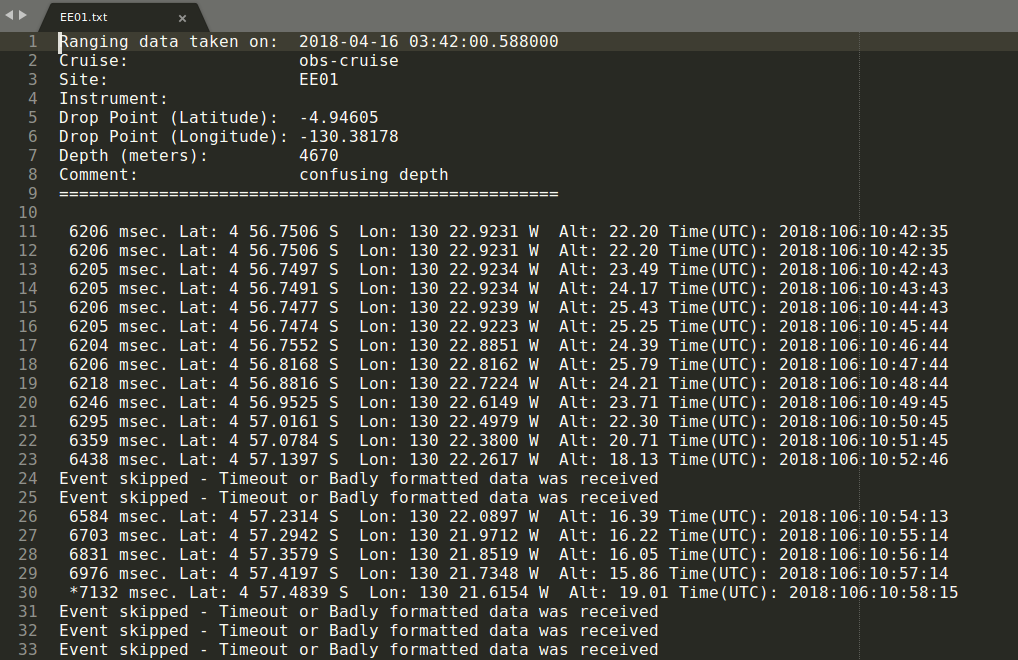
\includegraphics[width=\linewidth]{survey_fle_ex.png}
   \caption{Example survey \textit{.txt} file.}
   \label{fig:surveyfle}
  \end{figure} 
  
  \subsection{Coordinate System}
  During the sensor survey, whenever a ping is successfully received, the ship coordinates are logged as geodetic coordinates (latitude and longitude) using the ship's GPS. Such coordinates can be seen in Figure \ref{fig:surveyfle}. However \textit{\textbf{OBSrange}} (notably the inversion within) works with locally approximated Cartesian coordinates. The geodetic coordinates are converted in \textit{\textbf{OBSrange}} to a local Cartesian system (\textit{X},\textit{Y}) using the World Geodetic System 1984 (WGS84) reference ellipsoid. After the transformation is applied, the Cartesian origin ($X=0$, $Y=0$) of each individual survey pattern refers the corresponding instrument's drop location. 
  
  \subsection{Setting Parameters}
  \label{section:params}
  Slight design differences exist between the MATLAB and PYTHON versions of the code, but the main usage remains the same between the two. In both cases parameters are set in a single main script which will run and execute every other aspect of the code. Ideally, the only edits users ever need make are in editing the parameters of these main scripts. In the case of the MATLAB version, this script is called \textit{OBSrange.m} and these parameters are set in the top lines of that script. In the case of the PYTHON version, the main script is similarly called \textit{OBSrange.py}, and parameters are set in that script. The parameters to be set by users are described and compared in Table \ref{table:params} (sorted alphabetically by MATLAB parameter names).  Again, in both the MATLAB and PYTHON versions, once these parameters have been set, these scripts may be run and will produce results. 

  \newpage
  \begin{table}[H]
   \centering
   \caption{\textbf{\textit{OBSrange}} Parameter Descriptions.}
   \label{table:params}
   \footnotesize
   \begin{tabularx}{\linewidth}{|c|c|X|}
    \hline
    \textbf{MATLAB Parameter}   & \textbf{PYTHON Equivalent} & \textbf{Description} \\ \hline
    \textit{datapath}           & \textit{survey\_fles}      & Path to the directory containing the survey files.\\ \hline
    \textit{ifplot}             & \textit{-}                 & Option to plot results. In PYTHON plots are created and saved by default but not displayed when \textbf{\textit{OSBrange.py}} is run. In MATLAB plots are created, saved, and displayed while running \textbf{\textit{OBSrange.m}} if this parameter is set to 1.\\ \hline
    \textit{ifQC\_ping}         & \textit{QC}                & Option to perform quality control on ping results obtained from the survey files. Pings with two-way travel times beyond a certain threshold are filtered out of any analysis (see \textit{res\_thresh} below).\\ \hline
    \textit{ifsave}             & \textit{-}                 & By default the MATLAB version will write single station results to \textit{.txt} files. If this parameter is set to 1, then it will additionally write single station results to \textit{.mat} files. PYTHON writes single station results to both \textit{.pkl} and \textit{.txt} files by default.\\ \hline
    \textit{onesta}             & \textit{-}                 & Option to process a single station. PYTHON will process whatever survey files (\textit{.txt} files) are located in the directory represented by \textit{survey\_fles}.\\ \hline
    \textit{outdir}             & \textit{output\_dir}       & Path to output directory.\\ \hline
    \textit{par.dampdvp}        & \textit{dampdvp}           & Normal damping for water sound speed.\\ \hline
    \textit{par.dampx}          & \textit{dampx}             & Normal damping for station x-coordinate.\\ \hline
    \textit{par.dampy}          & \textit{dampy}             & Normal damping for station y-coordinate.\\ \hline
    \textit{par.dampz}          & \textit{dampz}             & Normal damping for station z-coordinate.\\ \hline
    \textit{par.dforward}       & \textit{dforward}          & GPS-transponder offset (meters). If unknown set to 0. Positive means the transponder is further forward than the GPS. \\ \hline
    \textit{par.dstarboard}     & \textit{dstarboard}        & GPS-transponder offset (meters). If unknown set to 0. Positive means the transponder is further starboard than the GPS. \\ \hline
    \textit{par.E\_thresh}      & \textit{E\_thresh}         & RMS reduction threshold for the inversion \\ \hline
    \textit{par.epsilon}        & \textit{eps}               & Global norm damping for stabilization.\\ \hline
    \textit{par.if\_raycorrect} & \textit{raycorr}           & Option to apply a travel time correction for ray-bending. If you choose to do this you can either provide your own sound speed profile for each station or our code will calculate one for you. See \textit{sspfile\_dir/ssp\_dir} below. \\ \hline
    \textit{par.if\_twtcorr}    & \textit{twtcorr}           & Option to apply a correction to two-way travel times due to the ship's radial velocity.\\ \hline
    \textit{par.N\_bs}          & \textit{N\_bs}             & Number of bootstrap iterations.\\ \hline
    \textit{par.npts\_movingav} & \textit{npts}              & Number of points in an N-point moving average smoothing filter applied to the ship's velocity. Note that if this parameter is set to “1” that no smoothing is applied. stuff\\ \hline
    \textit{par.sspfiledir}     & \textit{ssp\_dir}          & Path to directory of station sound speed profiles. If providing your own profiles, they \textbf{must} be named according to \textit{SSP\_stationname.txt}. \\ \hline
    \textit{par.TAT}            & \textit{tat}               & Turn-around time (\textit{msec}).\\ \hline
    \textit{par.vp\_w}          & \textit{vpw}               & Water velocity (\textit{m/s}).\\ \hline
    \textit{projpath}           & \textit{-}                 & Directory for both input and output (MATLAB only).\\ \hline
    \textit{res\_thresh}        & \textit{res\_thresh}       & Residual threshold for pings if applying quality control (\textit{msec}, see \textit{ifQC\_ping/QC} above).\\ \hline
   \end{tabularx}
  \end{table}

  \newpage
  \subsection{Structure}
   
   \begin{figure}[!htb]
    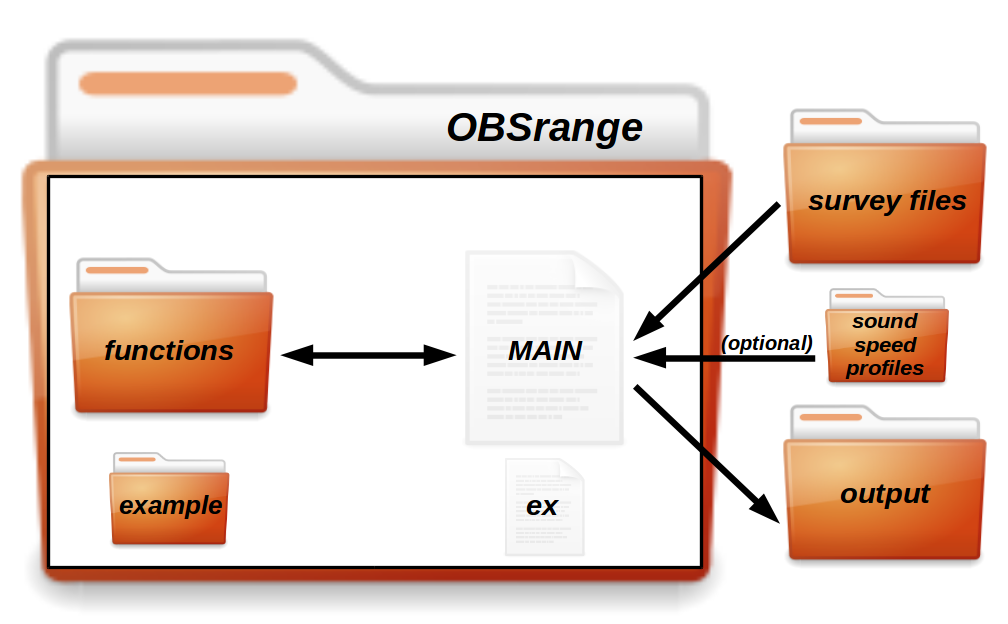
\includegraphics[width=\linewidth]{OBSrange_structure.png}
    \caption{\textbf{\textit{OBSrange}} structure.}
    \label{fig:struct}
   \end{figure}

   In this section we briefly describe the general structure of \textbf{\textit{OBSrange}},  illustrated in Figure \ref{fig:struct}. In both the MATLAB and PYTHON versions of the code, the top-level directory of \textbf{\textit{OBSrange}} includes the main script (\textit{OBSrange.m} or \textit{OBSrange.py}, respectively), in which the parameters for running the code are set by the user (see Section \ref{section:params}). Once parameters have been set, the main script can be run; it will loop through files in the survey files directory and call functions contained within the functions directory. All results will be written into an output directory. Note that paths to the directories for the survey files and output are specified by the user in the main script. In the case of the MATLAB version, these directories are themselves contained within a single folder, set via the \textit{projpath} variable. Finally, \textbf{\textit{OBSrange}} includes a single station example which will be discussed in the Section \ref{section:ex}.

 
 \section{Example}
 \label{section:ex}

  \subsection{General Output}
  The example provided with \textbf{\textit{OBSrange}} locates the OBS package deployed at site WC03 of the PacificORCA array (\textcolor{red}{reference}). Simply run the example script for your corresponding version of the code, either \textit{OBSrange\_example.py} or \textit{OBSrange\_example.m}. These scripts will read the example survey \textit{.txt} file contained within \textbf{\textit{OBSrange}}'s  example directory (see Figure \ref{fig:struct}) and will also write the output into that directory.  In the case of the PYTHON version, the output will consist of a \textit{.pkl} file named \textit{WC03\_location.pkl}, a \textit{.txt} file similarly named \textit{WC03\_location.txt}, and 6 figures. In the case of the MATLAB version the output will consist of a \textit{.txt} file also named \textit{WC03\_location.txt}, a \textit{.mat} file called \textit{WC03\_data.mat}, and the same figures.

  \subsection{The \textit{.txt} Files}
  The \textit{.txt} files created by the MATLAB and PYTHON versions are formatted slightly differently, but the results are the same. In Figure \ref{fig:ex} we show the first 40 lines of \textit{WC03\_location.txt} created by the PYTHON example and describe the general features of this file.\\

  \begin{figure}[!htb]
   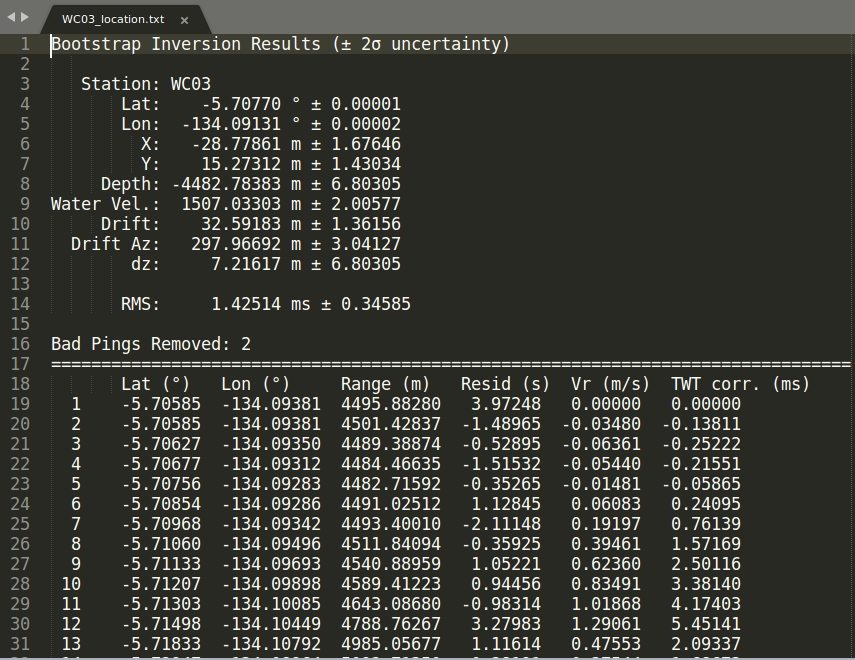
\includegraphics[width=\linewidth]{example_txt_fle.png}
   \caption{\textit{.txt} file output of \textit{OBSrange\_example.py}.}
   \label{fig:ex}
  \end{figure}

  In both versions, the header of \textit{WC03\_location.txt} summarizes the main results of the inversion performed by \textbf{\textit{OBSrange}} on this station. Shown in the header are the final estimates for the \textit{X} and \textit{Y} coordinates of the package relative to the drop point, as well as their converted latitude and longitude, and the final depth estimate (\textit{Depth}). Additionally, the header contains the total package drift distance (\textit{Drift}) and azimuth (\textit{Drift Az.}), the difference between the initial estimated depth and final depth estimate (\textit{dz}), and the depth averaged velocity of sound in water (\textit{Water Vel.}). Finally, the header contains the overall RMS misfit for this site and also displays the number of pings that were removed via the ping quality control. Below line 18 of \textit{WC03\_location.txt} the details of each ping are logged, namely, the ship latitude, longitude, estimated distance to the sensor, two-way travel-time residual, the ship's radial velocity and corresponding travel-time correction (whether it was applied or not).
 
  \subsection{The \textit{.pkl} and \textit{.mat} Files}
  In this example PYTHON will also create a \textit{.pkl} file called \textit{WC03\_out.pkl} and MATLAB will create a \textit{.mat} file called \textit{WC03\_out.mat}. In essence, both of these files are simply containers which hold various results of the bootstrap inversion. The \textit{.pkl} file contains a PYTHON \textit{dictionary} object of various results and values and the \textit{.mat} file contains a 1x1 \textit{struct} object called \textit{datamat}. Both data structures contain many of the same fields, all of which are listed in Table \ref{table:dict} (sorted alphabetically by MATLAB parameter names):

  \begin{table}[!htb]
   \centering
   \caption{Data fields contained in the \textit{.mat} and \textit{.pkl} files}
   \label{table:dict}
   \begin{tabularx}{\linewidth}{|c|c|X|}
    \hline
    \textbf{MATLAB} & \textbf{PYTHON} & \textbf{Description of Field} \\ \hline
    -               & dzs        & The depth difference after each bootstrap iteration. \\ \hline
    azi\_bs         & azs        & Sensor drift azimuth after each bootstrap iteration. \\ \hline
    Cm\_mat         & cov        & Model covariance matrices after each bootstrap iteration. \\ \hline
    databad         & Nbad       & The number of pings removed via quality control. \\ \hline
    drift\_bs       & drifts     & Sensor drift distance after each bootstrap iteration. \\ \hline
    drop\_lonslatz  & drop\_geo  & Geographic drop coordinates. \\ \hline
    dtwt\_bs        & dtwts      & Final twtt residuals at each survey point. \\ \hline
    dtwtcorr\_bs    & corrs      & Final twtt corrections at each survey point (whether applied or not). \\ \hline
    E\_rms          & E\_rms     & RMS after each bootstrap iteration. \\ \hline
    Ftest\_res      & Ftest\_res & F-test grid search results. \\ \hline
    lat\_sta\_bs    & lat\_sta   & Sensor latitude after each bootstrap iteration. \\ \hline
    lats\_ship      & svy\_lats  & Latitudes of survey points. \\ \hline
    loc\_lolaz      & loc\_geo   & Final sensor location (geographic coordinates). \\ \hline
    loc\_xyz        & loc\_xyz   & Final sensor location (Cartesian reference frame). \\ \hline
    lon\_sta\_bs    & lon\_sta   & Sensor longitude after each bootstrap iteration. \\ \hline
    lons\_ship      & svy\_lons  & Longitudes of survey points. \\ \hline
    mean\_drift\_az & drift\_az  & Final sensor drift distance and azimuth. \\ \hline
    R\_mat          & resol      & Model resolution matrices after each bootstrap iteration. \\ \hline
    sta             & sta        & Station name. \\ \hline
    TAT\_bs         & tats       & Sensor turn-around time after each bootstrap iteration. \\ \hline
    twtcorr\_bs     & twts       & Final two-way travel-times (twtts) at each survey point. \\ \hline
    x\_ship         & svy\_xs    & x-coordinates of ship at each survey point. \\ \hline
    x\_sta\_bs      & x\_sta     & x-coordinates of sensor after each bootstrap iteration. \\ \hline
    y\_ship         & svy\_ys    & y-coordinates of ship at each survey point. \\ \hline
    y\_sta\_bs      & y\_sta     & x-coordinates of sensor after each bootstrap iteration. \\ \hline
    z\_ship         & svy\_zs    & z-coordinates of ship at each survey point. \\ \hline
    z\_sta\_bs      & z\_sta     & x-coordinates of sensor after each bootstrap iteration. \\ \hline
    v\_ship         & svy\_vs    & Ship velocity at each survey point. \\ \hline
    \end{tabularx}
   \end{table}
  
  \newpage

  \subsection{Figures}
  In conclusion we show the figures produced after running \textit{\textbf{OBSrange.py}} for the above example.

  \begin{figure}[!htb]
   \centering
   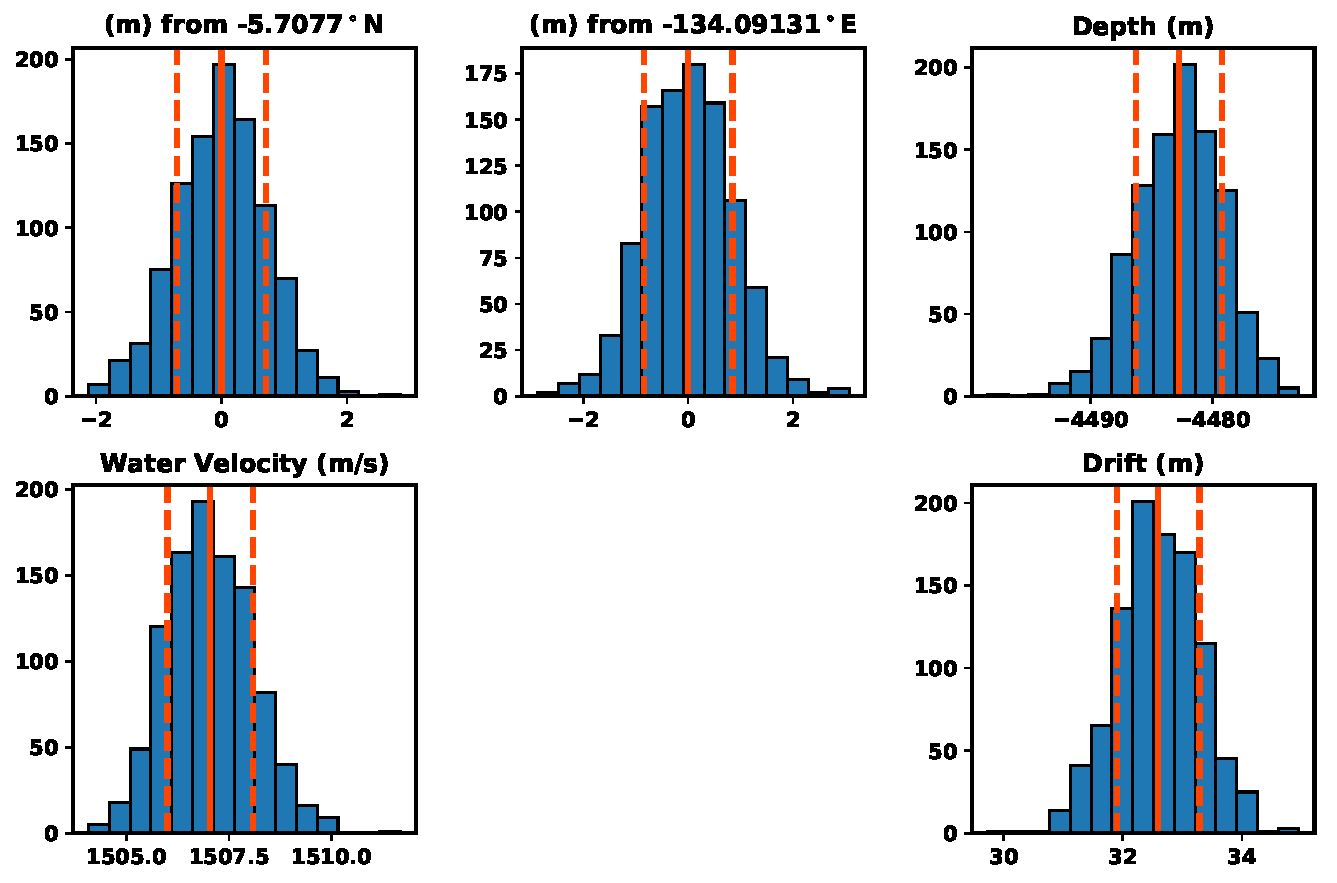
\includegraphics[width=0.8\linewidth]{histograms.pdf}
   \caption{Model parameter histograms.}
  \end{figure}

  \begin{figure}[!htb]
   \centering
   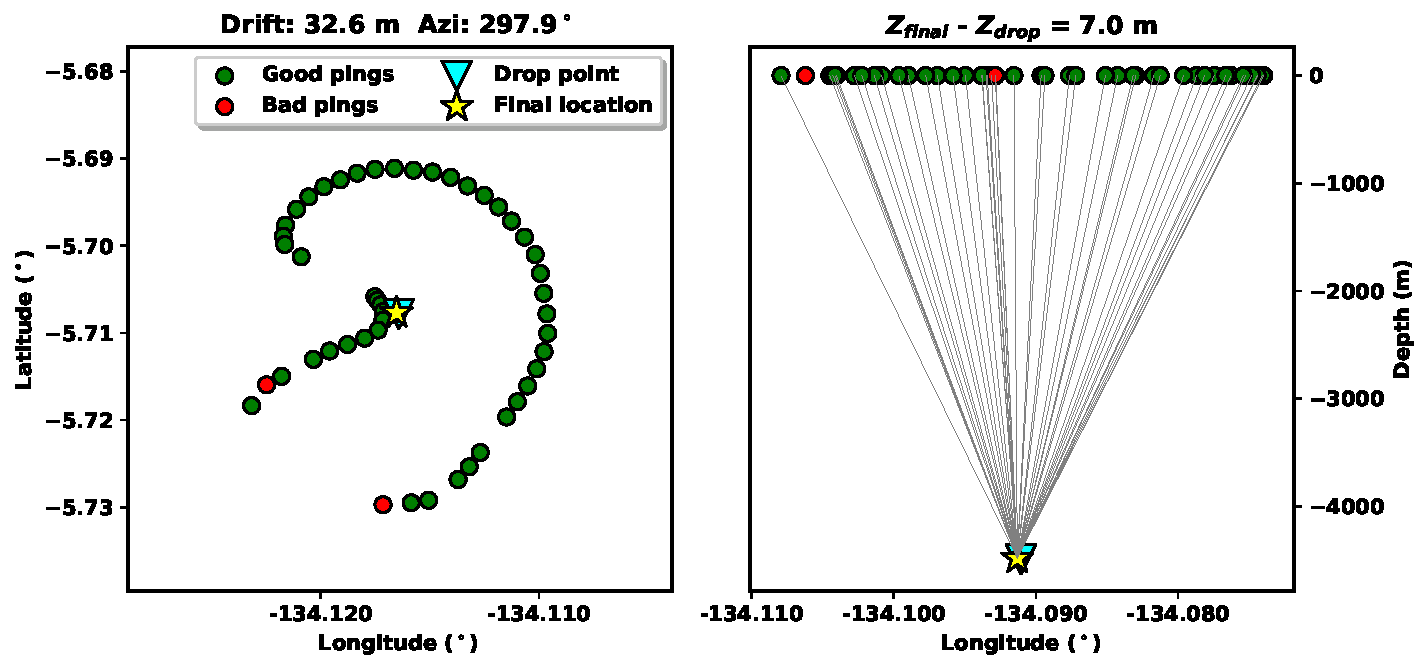
\includegraphics[width=0.9\linewidth]{maps.pdf}
   \caption{Survey maps.}
  \end{figure}
 
  \begin{figure}[!htb]
   \centering
   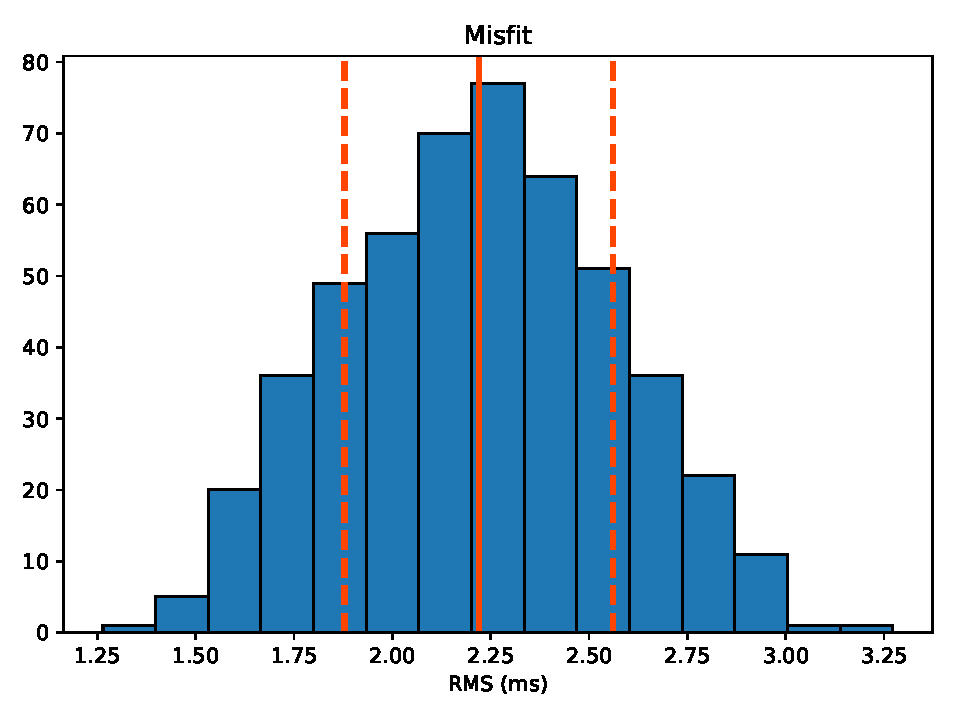
\includegraphics[width=0.7\linewidth]{misfit.pdf}
   \caption{Final model misfit.}
  \end{figure}

  \begin{figure}[!htb]
   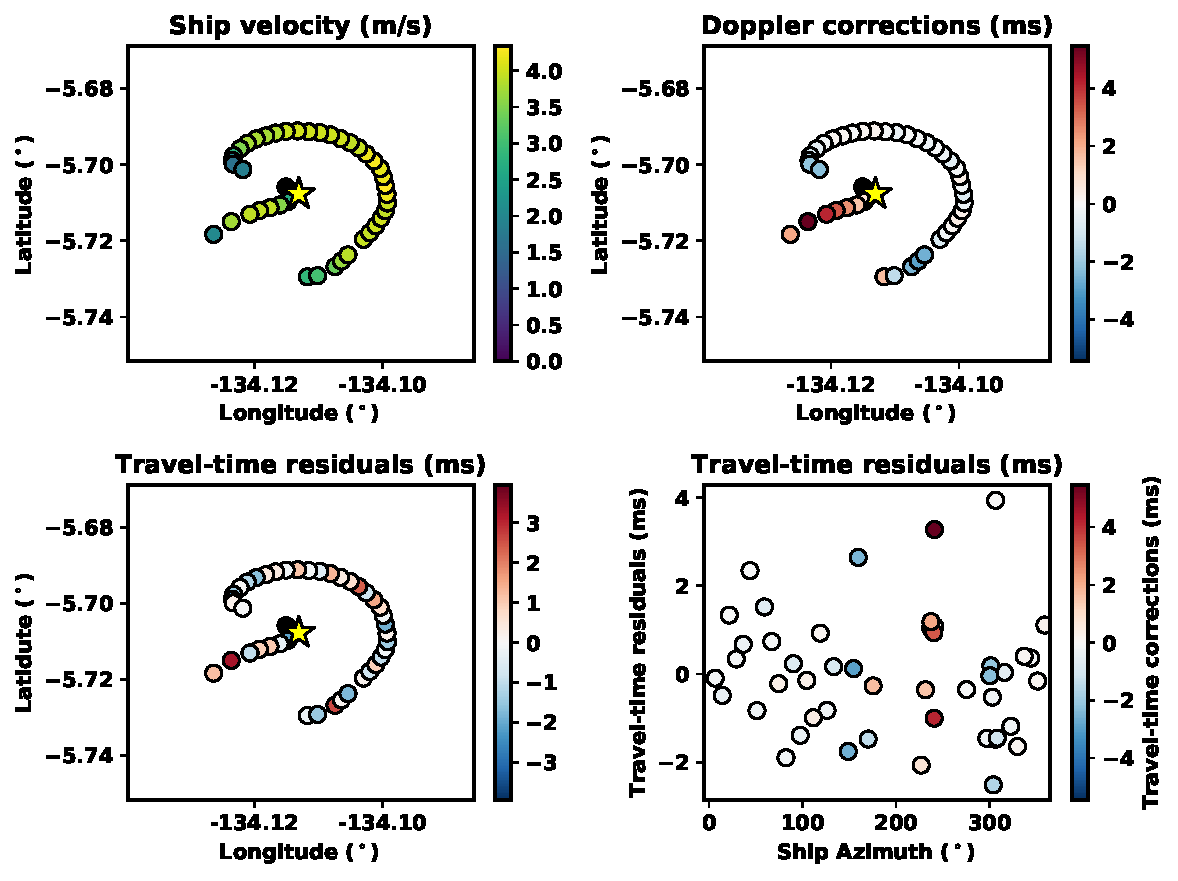
\includegraphics[width=\linewidth]{tt_resids.pdf}
   \caption{Two-way travel-time residuals by suvery point}
  \end{figure}
  
  \begin{figure}[!htb]
   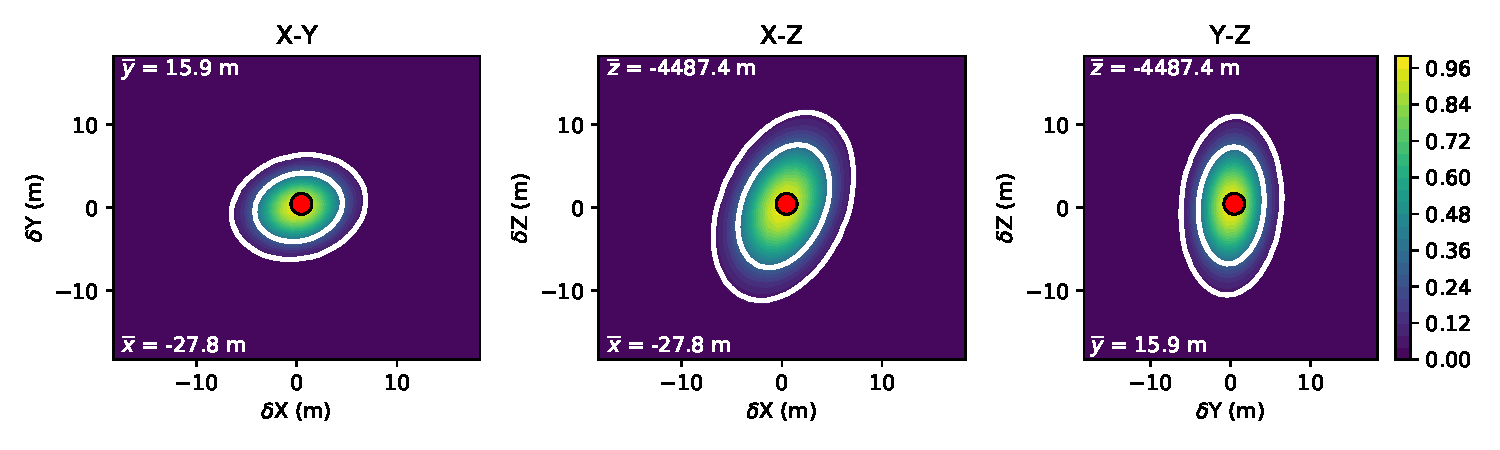
\includegraphics[width=\linewidth]{ftest.pdf}
   \caption{F-test derived location uncertainty}
  \end{figure}
  
  \begin{figure}[!htb]
   \centering
   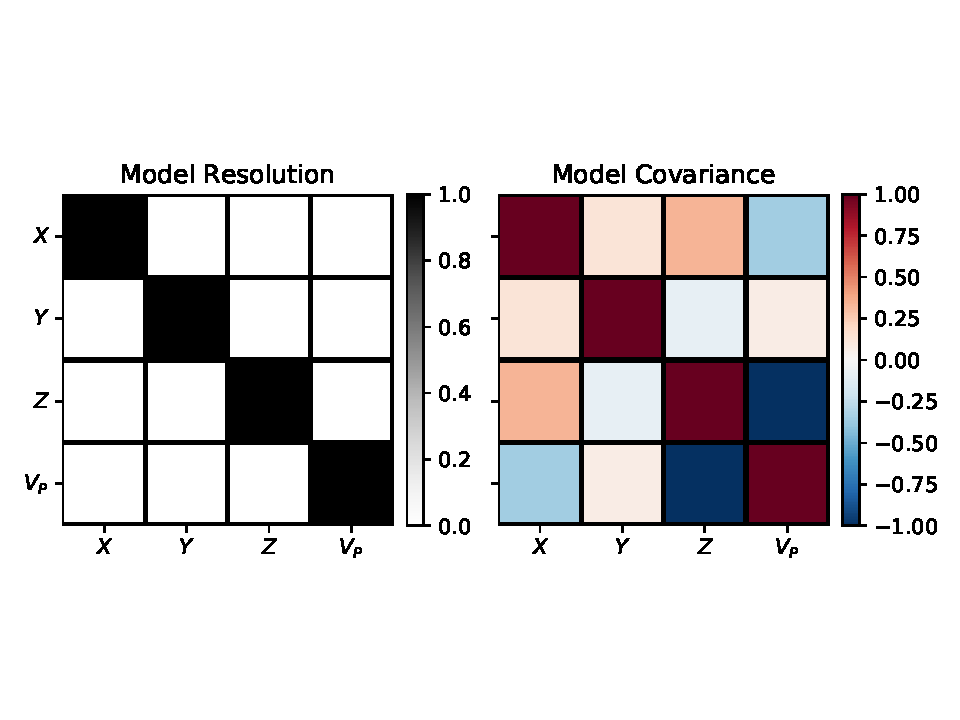
\includegraphics[width=0.9\linewidth]{resolution_matrices.pdf}
   \caption{Final model desolution and covariance}
  \end{figure}

 \section*{References}
 \addcontentsline{toc}{section}{References}
 \textcolor{red}{Our paper.}

\end{document}